\documentclass{beamer}
\usepackage{animate}
\usepackage[export]{adjustbox}
\usepackage{amsmath,amsfonts,amsthm,bm} % Math packages

\usetheme{CambridgeUS}

\title[Some RBF-FD properties]{Some properties of RBF-FD differential operator approximations}
\author[Andrej Kolar - Po{\v z}un]{Doctoral dissertation proposal \linebreak\linebreak Author: Andrej Kolar-Po{\v z}un \linebreak Mentor: Dr. Gregor Kosec }
\institute[]{Jožef Stefan Institute \linebreak University of Ljubljana - Faculty of Mathematics and Physics}
\begin{document}
\begin{frame}
\titlepage
\end{frame}
\begin{frame}
\frametitle{Numerical treatment of PDEs - Finite Difference Method}
\begin{itemize}
\item<1-> Goal: Solve $\mathcal{L} u(x) = f(x), x \in \Omega$ (and boundary conditions)
\item<2-> Step 1 - discretise $\Omega$ to obtain a (regular) discretisation $\{x_i\}_i \subset \Omega$.
\item<3-> Step 2 - approximate the operator $\mathcal{L}$ locally (i.e. 5-point, 9-point stencil,..).
\item<4-> Step 3 - Form a linear system by requiring the discretised PDE to hold at each $x_i$.
\item<5-> Step 4 - Invert the system to obtain the values $u(x_i)$.
\end{itemize}
\end{frame}

\begin{frame}
\frametitle{RBF-FD - Radial Basis Function generated Finite Differences}
\begin{itemize}
\item<1-> Strong-form meshless methods: $\{ x_i \}_i \subset \Omega$ can be irregular.
\item<2-> RBF-FD provides an approximation of the form $\mathcal{L} u(x_i) \approx \sum_{j \in S_i} w_j u(x_j)$.
\end{itemize}
\onslide<3->\begin{equation*}
\begin{pmatrix} A & P \\
P^T & 0
\end{pmatrix}
\begin{pmatrix}
w \\
\lambda
\end{pmatrix}
=
\begin{pmatrix}
\mathcal{L}(\phi) \\
\mathcal{L}(p)
\end{pmatrix}
\end{equation*}

\onslide<3->\begin{equation*}
A = \begin{pmatrix} 
    \phi(||x_1-x_1||) & \dots  & \phi(||x_1-x_n||)\\
    \vdots & \ddots & \vdots\\
    \phi(||x_n - x_1||) & \dots  & \phi(||x_n-x_n||) 
    \end{pmatrix}
\end{equation*}
\onslide<3->\begin{equation*}
P = \begin{pmatrix} 
    p_1(x_1) & \dots  & p_M(x_1)\\
    \vdots & \ddots & \vdots\\
    p_1(x_n) & \dots  & p_M(x_n)  
    \end{pmatrix}
\end{equation*}

\end{frame}

\begin{frame}
\frametitle{Example meshless discretisation}
\includegraphics[width=.6\linewidth,center]{Figures/Discretisation.png}
\end{frame}

\begin{frame}
\frametitle{Some further properties of RBF-FD}
\begin{itemize}
\item<1-> RBFs allow for interpolation on scattered data with provable invertibility guarantees.
\item<2-> RBF-FD approximation is obtained by applying $\mathcal{L}$ to the interpolant.
\item<3-> Polyharmonic Spline (PHS) RBF: $\phi(r) = r^3$ - no shape parameter, improved stability.
\item<4-> Monomial augmentation of order $m$ - Polynomial reproduction up to order $m$.
\end{itemize}
\end{frame}

\begin{frame}
\frametitle{Core topics}
\begin{itemize}
\item<1-> Oscillatory behaviour of RBF-FD error under increasing stencil size.
\item<2-> Superconvergent behaviour of the RBF-FD method.
\item<3-> The "RBF FDM".
\item<4-> Smoothness of the RBF-FD approximation.
\end{itemize}
\end{frame}

\begin{frame}
\frametitle{Typical research strategy}
\begin{itemize}
\item<1-> Simple problem (circular domain, $\nabla^2 u(x,y) = f(x,y)$, Dirichlet BC)
\item<2-> Choose a function $u(x,y)$ and solve the corresponding PDE with RBF-FD
\item<3-> Study the error behaviour and the approximation properties.
\end{itemize}
\end{frame}

\begin{frame}
\frametitle{Oscillatory behaviour of RBF-FD error under increasing stencil size}
\begin{itemize}
\item<1-> $u(x,y) = \sin (\pi x) \sin (\pi y)$.
\item<2-> Fix monomial augmentation $m=3$, $h=0.01$, $\phi(r) = r^3$, increase the stencil size and observe that the solution error oscillates.
\end{itemize}
\visible<2->{\includegraphics[width=.8\linewidth,center]{Figures/MeanErrors.png}}
\end{frame}
\begin{frame}
\frametitle{Oscillatory behaviour of RBF-FD error under increasing stencil size}
\begin{itemize}
\item Oscillatory error can be connected to the pointwise error behaviour.
\end{itemize}
\includegraphics[width=.8\linewidth,center]{Figures/PlotWithContours.png}
\end{frame}

\begin{frame}
\frametitle{Oscillatory behaviour of RBF-FD error under increasing stencil size}
\begin{itemize}
\item Quantity $\delta N_\mathrm{poiss}^\pm$ ("mean sign of pointwise error") - minima indicator?
\end{itemize}
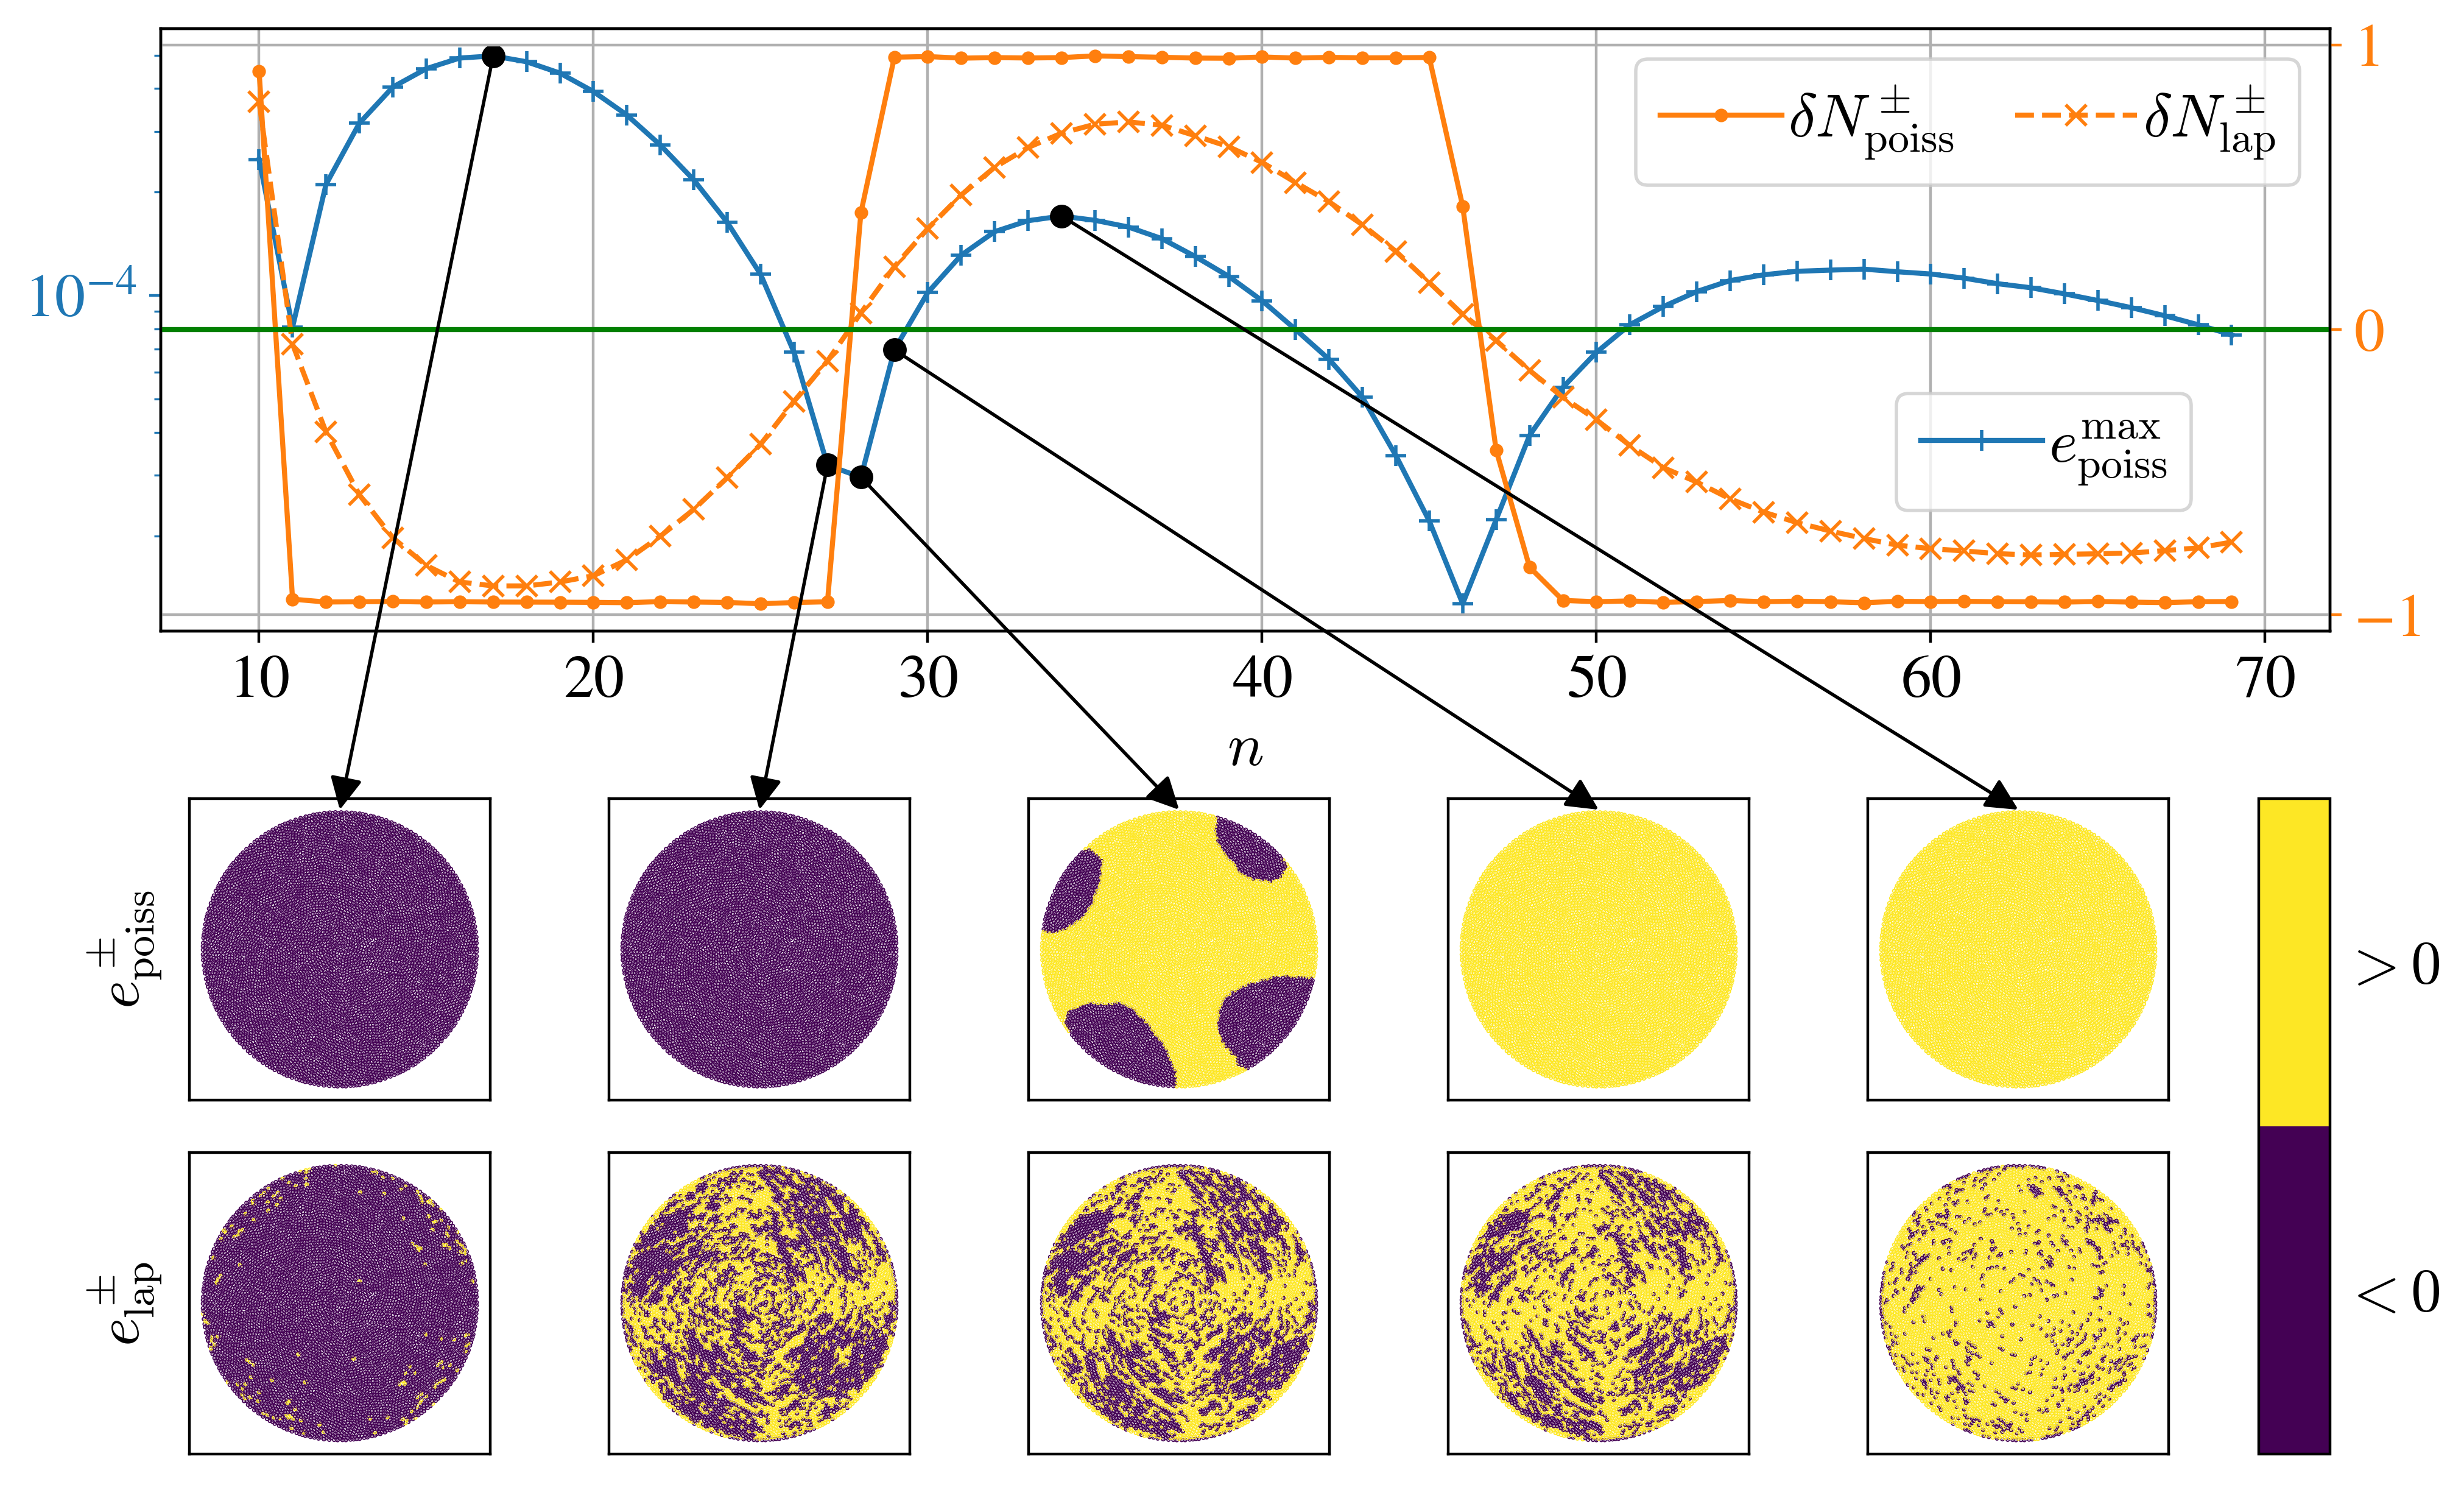
\includegraphics[width=.7\linewidth,center]{Figures/MetricContours.png}
\end{frame}

\begin{frame}
\frametitle{Oscillatory behaviour of RBF-FD error under increasing stencil size}
\begin{itemize}
\item The behaviour is robust under various different changes of the problem setup and method parameters.
\end{itemize}
\includegraphics[width=.8\linewidth,center]{Figures/DifferentDomains.png}
\end{frame}

\begin{frame}
\frametitle{Oscillatory behaviour of RBF-FD error under increasing stencil size}
\begin{itemize}
\item ... But there are exceptions.
\end{itemize}
\begin{table}
\centering
\begin{tabular}{|c |c |}
 \hline
 Label & $u(x,y)$ \\ 
 \hline\hline
 $u_1$ & $x^4 y^5$ \\ 
\hline
 $u_2$ & $1+\sin(4x) + \cos(3x) + \sin(2y)$  \\ 
\hline
 $u_3$ & $\exp(x^2)$  \\ 
\hline
 $u_4$ & $\mathrm{arsinh}(x+2y)$  \\ 
\hline
 $u_5$ & $\cos(\pi x)\cos(\pi y)$  \\ 
\hline
 $u_6$ & $\mathrm{franke}(x,y)$ \\ 
\hline
\end{tabular}
\end{table}
\end{frame}

\begin{frame}
\frametitle{Oscillatory behaviour of RBF-FD error under increasing stencil size}
\includegraphics[width=.8\linewidth,center]{Figures/DifferentFunctions.png}
\end{frame}


\begin{frame}
\frametitle{Superconvergence of the RBF-FD method}
\begin{itemize}
\item<1-> Solve the Poisson equation with $u(x,y) = 1 + \sin(4x) + \cos(3x) + \sin(2y)$.
\item<2-> Calculate the error dependence on $h$ (over different discretisations)
\item<3-> Operator approximation order matches theory - $h^{m-1}$ ($h^{m+1-k}$).
\item<3-> Solution order is $h^{m-1}$ or $h^m$
\end{itemize}
\visible<2->{\includegraphics[width=.8\linewidth,center]{Figures/convergenceAll.png}}
\end{frame}

\begin{frame}
\frametitle{Superconvergence of the RBF-FD method}
\begin{itemize}
\item<1-> The solution error can be obtained as a solution to $A e_\mathrm{sol} = e_\mathrm{op}$.
\item<2-> The form of $e_\mathrm{op}$ is actually known\only<2->{\footnote{Bayona V., An insight into RBF-FD approximations augmented with monomials, 2019}}:
\item<2-> $\nabla^2\hat{u}(x_i,y_i) - \nabla^2u(x_i,y_i) = \sum_{k=s+1}^\infty L_k [u(x_i,y_i)] (\textbf{p}_k^T \cdot \textbf{w})$.
\item<3-> Study the error behaviour term by term in powers of $h$.
\end{itemize}
\visible<3->{\includegraphics[width=.8\linewidth,center]{Figures/errorFormula.png}}
\end{frame}



\begin{frame}
\frametitle{RBF FDM}
\begin{itemize}
\item<1-> "Radial Basis Function Finite Difference Method".
\item<2-> Employing RBF interpolants, interpolate scattered nodes to a "{} virtual "{} FDM stencil and apply FDM formulas.
\item<2-> Already sucessfuly applied to physical problems\only<2->{\footnote{Vuga G., Mavrič B. and Šarler B., An improved local radial basis function method for solving small-strain elasto-plasticity, 2024}}
\item<3-> New parameters - shape and spacing of the "{}virtual"{} FDM stencil.
\end{itemize}
\visible<2->{\includegraphics[width=.7\linewidth,center]{Figures/fdm.png}}
\end{frame}

\begin{frame}
\frametitle{RBF-FDM applications}
\visible<1->{\includegraphics[width=.6\linewidth,center]{Figures/fdmresults.png}}
\end{frame}

\begin{frame}
\frametitle{RBF FDM motivation}
\begin{itemize}
\item<1-> Greater stability under decreasing $h$.
\item<2-> Potentially better suited for problems with discontinuity.
\item<3-> Sometimes a grid may also be desired, i.e. Yee's algorithm.
\end{itemize}
\end{frame}






\begin{frame}
\frametitle{Smoothness of the approximation}
\begin{itemize}
\item<1-> The usual error estimates assume the solution in question is sufficiently smooth.
\item<2-> In a numerical setting, a similar notion is well-resolvedness of a function.
\item<3-> Taylor series remainder - $\propto f^{(p+1)}(\xi) h^{p+1}$
\item<4-> For a badly resolved function, increasing the method order is undesirable!
\item<5-> Main question - when should the order be increased?
\end{itemize}
\end{frame}

\begin{frame}
\frametitle{Smoothness of the approximation - Application and Motivation}
\begin{itemize}
\item<1-> hp refinement - iterative spatial modification of nodal density (h-) and method order (p-)\only<1->{\footnote{Jančič M. and Kosec G., Strong form mesh-free hp-adaptive solution of linear elasticity problem, 2023}}.
\item<2-> h-refining should be preferred in the areas, where the solution is less smooth - smoothness indicator?
\item<3-> Connection with RBFs.
\end{itemize}
\visible<1->{\includegraphics[width=.7\linewidth,center]{Figures/hprefinement.png}}
\end{frame}


\begin{frame}
\frametitle{Summary}
\begin{itemize}
\item<1-> Our work aims to further the understanding of PHS RBF-FD approximations.
\item<2-> We aim to analyse the two observed behaviours - oscillating error and order elevation. 
\item<3-> We plan to systematically research the RBF FDM.
\item<4-> We wish to incorporate solution smoothness information in the solution procedure.
\end{itemize}
\end{frame}

\end{document}